\documentclass[12pt,a4paper]{amsart}
\usepackage[slovene]{babel}
%\usepackage[cp1250]{inputenc}
\usepackage[T1]{fontenc}
\usepackage[utf8]{inputenc}
\usepackage{amsmath,amssymb,amsfonts}
\usepackage{url}
\usepackage[normalem]{ulem}
\usepackage[dvipsnames,usenames]{color}
\usepackage{graphicx}

% Oblika strani
\textwidth 15cm
\textheight 24cm
\oddsidemargin.5cm
\evensidemargin.5cm
\topmargin-5mm
\addtolength{\footskip}{10pt}
\pagestyle{plain}
\overfullrule=15pt % oznaci predlogo vrstico

% Ukazi za matematična okolja
\theoremstyle{definition} % tekst napisan pokončno
\newtheorem{definicija}{Definicija}[section]
\newtheorem{primer}[definicija]{Primer}
\newtheorem{opomba}[definicija]{Opomba}

\renewcommand\endprimer{\hfill$\diamondsuit$}


\theoremstyle{plain} % tekst napisan poševno
\newtheorem{lema}[definicija]{Lema}
\newtheorem{izrek}[definicija]{Izrek}
\newtheorem{trditev}[definicija]{Trditev}
\newtheorem{posledica}[definicija]{Posledica}

\begin{document}

%%%%%%%%%%%%%%%%%%%%%%%%%%%%%%%%%%%%%%%%%%%%%%%%%%%%%%%%%%%%%%%%%%%%%%%%%%%%%%%%%%%%%%%%%%%%%%%%%%%%%%%%%%%%%%%%%%%%%%%%%%%%%%%%%%%%%%%%%%%%%%
\title{Statistika v kazenskem pravu}
\author{Neža Kržan}
\maketitle

%%%%%%%%%%%%%%%%%%%%%%%%%%%%%%%%%%%%%%%%%%%%%%%%%%%%%%%%%%%%%%%%%%%%%%%%%%%%%%%%%%%%%%%%%%%%%%%%%%%%%%%%%%%%%%%%%%%%%%%%%%%%%%%%%%%%%%%%%%%%%%
%%%%%%%%%%%%%%%%%%%%%%%%%%%%%%%%%%%%%%%%%%%%%%%%%%%%%%%%%%%%%%%%%%%%%%%%%%%%%%%%%%%%%%%%%%%%%%%%%%%%%%%%%%%%%%%%%%%%%%%%%%%%%%%%%%%%%%%%%%%%%%
\section{Statistika v kazenskem pravu}
Raziskave na področju kazenskega pravosodja in kriminologije so različne po naravi in namenu. Velik del raziskav vključuje preverjanje teorije in hipotez. 
Teorije so predlagane razlage določenih dogodkov. Hipoteze so majhni deli teorij, ki morajo biti resnični, da bi celotna teorija držala. Teorijo 
si lahko predstavljamo kot verigo, hipoteze pa kot člene, ki sestavljajo to verigo.\\\\
Raziskovalci na področju kazenskega pravosodja in kriminologije si običajno prizadevajo preučiti razmerja med dvema ali več spremenljivkami. Opazovani 
ali empirični pojavi sprožajo vprašanja.\\\\
Odvisne spremenljivke so empirični dogodki, ki jih želi raziskovalec pojasniti. Primeri odvisne spremenljivke so stopnje umorov, stopnje premoženjskih 
kaznivih dejanj, povratništvo med nedavno izpuščenimi zaporniki in sodne odločitve o izreku kazni. Raziskovalci skušajo opredeliti spremenljivke, 
ki pomagajo napovedati ali pojasniti te dogodke. Neodvisne spremenljivke so dejavniki, za katere raziskovalec meni, da bi lahko vplivali na odvisne 
spremenljivke. Glede na naravo raziskovalne študije določimo neodvisne in odvisne spremenljivke.\\\\
Pomembno je razumeti, da neodvisno in odvisno nista sinonima za vzrok in posledico. Določene neodvisne spremenljivke so lahko povezane z določenimi 
odvisnimi spremenljivkami, vendar to še zdaleč ni dokončen dokaz, da so prve vzrok drugih. Za dokazovanje vzročnosti morajo raziskovalci dokazati, 
da njihove študije izpolnjujejo tri merila. Prvo je časovno zaporedje, kar pomeni, da se mora neodvisna spremenljivka pojaviti pred odvisno spremenljivko. 
Druga zahteva glede vzročnosti je, da obstaja empirična povezava med neodvisno spremenljivko in odvisno spremenljivko. Zadnja zahteva je, da je razmerje 
med neodvisno spremenljivko in odvisno spremenljivko nepristransko. orej vse vrste spremenljivk so med seboj povezane, vendar je pomembno, da na 
podlagi statističnih povezav ne sklepamo prehitro o vzročnih posledicah, kar pa bi lahko bila težava.\\\\
Statistični znanstveniki se že na začetku sodnega procesa soočajo s prvimi težavami - določitvijo odvisnih in neodvisnih spremenljivk za modeliranje. V 
proces določanja spremenljivk pa pogosto posežejo odvetniki, ki se sklicujejo na pravne zakone in načela. To lahko postane sporno, saj lahko takšni 
posegi ovirajo statistične znanstvenike pri izračunu verjetnostnega vpliva spremenljivk. Odvetniki imajo pomembno vlogo pri zagovarjanju strank v 
sodnih postopkih, vendar je njihovo znanje o statistiki in verjetnostnih izračunih omejeno. Po mojem mnenju zato odvetniki lahko napačno opredelijo 
odvisne in neodvisne spremenljivke ter s tem vplivajo na kakovost modeliranja. To pa lahko privede do napačnih zaključkov in napravilnih odločitev v 
sodnih postopkih. Zato menim, da je sodelovanje med statistični znanstveniki in odvetniki pomembno. S tem se lahko zagotovi pravilno opredelitev 
spremenljivk in pravilne verjetnostne izračune, ki bodo prispevali k pravičnim odločitvam v sodnih postopkih.

%%%%%%%%%%%%%%%%%%%%%%%%%%%%%%%%%%%%%%%%%%%%%%%%%%%%%%%%%%%%%%%%%%%%%%%%%%%%%%%%%%%%%%%%%%%%%%%%%%%%%%%%%%%%%%%%%%%%%%%%%%%%%%%%%%%%%%%%%%%%%%
%%%%%%%%%%%%%%%%%%%%%%%%%%%%%%%%%%%%%%%%%%%%%%%%%%%%%%%%%%%%%%%%%%%%%%%%%%%%%%%%%%%%%%%%%%%%%%%%%%%%%%%%%%%%%%%%%%%%%%%%%%%%%%%%%%%%%%%%%%%%%%
\section{Uporaba statistike pri pravnem postopku}
Pri skoraj vseh uporabah podatkov se sodni postopek zanaša na razlago strokovnjakov, ki ocenijo zanesljivost podatkovne baze in pravilno razlagajo 
rezultate statistične analize. Pred pričanjem na sodišču moramo vedeti, 
na kaj točno se podatki nanašajo, kako so bili zbrani in kakšen del manjka ali je neuporaben, da se lahko odločimo za ustrezen postopek analize podatkov.
Potrebujemo osnovne informacije odvetnika in drugih strokovnjakov, da lahko oblikujemo ustrezne primerjalne skupine. Ta postopek vključuje 
določitev ustrezne populacije (populacij), ki jo (jih) je treba preučiti, parametrov, ki nas zanimajo, in statističnega postopka, ki ga je treba uporabiti. 
Statistiki ne morejo določiti, katere vrednosti parametra so pravno pomembne, ker je parameter pravno določen.\\\\
Statistične informacije, ki jih dobi sodnik, so filtrirane prek odvetnikov. Odvenik avtorju statistične analize postavlja vprašanja z namenom razlage 
statistične analize poroti, sodniku in drugim v sodni dvorani. Vprašanja so s strani odvetnikov seveda premišljeno postavljena, zato se lahko zgodi, da do 
temeljite razlage analize ne pride, ker analitik ne dobi primernih vprašanj. Kasneje bom obrazložila zmote, ki nastanejo zaradi pomankanja znanja verjetnosti 
pri sodnikih, poroti in odvetnikih, mogoče pa nekatere izmed njih nastanejo tudi zaradi nepopolne razlage statistične analize. Do neke točke analitik sicer sam 
predstavi analizo, potem pa mora biti tudi on previden z razlago, zaradi porote, kajti poroti se predvidoma ne govori kako naj si razlaga dokaze, kar pa ponavadi preučujemo 
s statistično analizo. Mogoče bi moralo biti določeno kaj vse mora analitik predstaviti in razložiti, da bi se lahko izognili zmotam.\\
Uporaba statističnih analiz na sodiščih prinaša tudi nove težave za statistiko. Temelj dobre statistične analize je dober pregled predpostavk, na 
katerih morajo temeljiti naše metode in upoštevanje pravil prava. Pomembne so tudi baze podatkov in velikosti vzorcev, kar lahko predstavlja težavo. 
Potrebno je kombiniranje različnih postopkov za pridobivanje informacij iz podatkov in razlago rezultatov, kar sem zasledila, da strokovnjaki velikokrat 
izkoriščajo, se ne poglobijo dovolj in predstavljena analiza postane nepopolna.

%%%%%%%%%%%%%%%%%%%%%%%%%%%%%%%%%%%%%%%%%%%%%%%%%%%%%%%%%%%%%%%%%%%%%%%%%%%%%%%%%%%%%%%%%%%%%%%%%%%%%%%%%%%%%%%%%%%%%%%%%%%%%%%%%%%%%%%%%%%%%%
%%%%%%%%%%%%%%%%%%%%%%%%%%%%%%%%%%%%%%%%%%%%%%%%%%%%%%%%%%%%%%%%%%%%%%%%%%%%%%%%%%%%%%%%%%%%%%%%%%%%%%%%%%%%%%%%%%%%%%%%%%%%%%%%%%%%%%%%%%%%%%
\section{Raziskovalni proces}
Raziskovalni proces v kazenskem pravosodju je običajno namenjen preučevanju problemov kriminala. Proces se izvaja po naslednjih točkah.\\
\textit{1. Identifikacija problema.\\} 
\textit{2. Zasnova raziskave.\\} 
\textit{3. Analiza podatkov.\\}

%%%%%%%%%%%%%%%%%%%%%%%%%%%%%%%%%%%%%%%%%%%%%%%%%%%%%%%%%%%%%%%%%%%%%%%%%%%%%%%%%%%%%%%%%%%%%%%%%%%%%%%%%%%%%%%%%%%%%%%%%%%%%%%%%%%%%%%%%%%%%%
%%%%%%%%%%%%%%%%%%%%%%%%%%%%%%%%%%%%%%%%%%%%%%%%%%%%%%%%%%%%%%%%%%%%%%%%%%%%%%%%%%%%%%%%%%%%%%%%%%%%%%%%%%%%%%%%%%%%%%%%%%%%%%%%%%%%%%%%%%%%%%
\section{Vrednotenje dokazov}
Ena od najbolj obravnavanih in kontroverznih tem med pravniki je vloga verjetnosti pri ocenjevanju pravnih dokazov, pridobljenih v postopku 
ugotavljanja dejstev in preiskave, ki je značilen za sodišča. Na mednarodnih kazenskih sodiščih je vodilno načelo prosta ocena dokazov, kar pomeni, 
da sodniki niso dolžni spoštovati pravil, kako ocenjevati dokaze, in zato lahko izberejo pristop, ki naj bi bil najprimernejši za oceno.\\
Postopek ugotavljanja dejstev zahteva oceno vseh dokazov, ki jih predložijo sodišču, da se določi, ali je obdolženec kriv 
ali ne. Uvede se pojem dokazni standard, ki je pravno vprašanje, tj. gre za abstraktno normo, ki je (podobno kot obstoj določenih predpostavk za 
določeno kaznivo dejanje) opredeljena s pravnim pravilom. Vrednotenje dokazov pa je t.i. dejansko vprašanje, gre za odločitev, kako se dokazi, v določenem 
primeru, nanašajo na normo. \\\\
Matematični pristopi za ocenjevanje dokazov določajo različne odstotke za dokazni standard, ki je manjši od popolne gotovosti, zato se 
predložene informacije (ali njihovo pomanjkanje) pretvorijo v številčno vrednost (običajno približno 90-95-odstotna stopnja verjetnosti), ki se nato 
primerja z zahtevanim dokaznim standardom.\\\\
Najpogostejši uporabljeni metodi za ocenjevanje dokazov sta metoda dokazne vrednosti in model verjetnosti hipoteze. Metoda dokazne vrednosti temelji na vrednosti, ki 
jo ima dokaz za dokazno temo, njen namen pa je ugotoviti, ali med dokazom in zadevno dokazno temo obstaja naključna povezava. S to metodo dokazujemo 
določen omejen nabor dokazov, njen cilj pa je oceniti verjetnost, da dokazi dokazujejo hipotezo. Cilj modela 
verjetnosti hipoteze pa je oceniti verjetnost hipoteze glede na dokaze. Cilj je ugotoviti, kako verjetno je, da je hipoteza, za katero dokazi 
lahko zagotavljajo določeno stopnjo podpore ali ne, resnična. Glavna razlika z metodo dokazne vrednosti je, da predpostavlja, da obstaja začetna 
verjetnost za hipotezo pred obravnavo dokazov, t.i. predhodna verjetnost.\\\\
V kazenskem pravu pa lahko zelo hitro pride do posebnih, edinstvenih predpostavk oziroma hipotez, ki pa predstavljajo težave pri vrednotenju oziroma 
merjenju v statističnih modelih. 

%%%%%%%%%%%%%%%%%%%%%%%%%%%%%%%%%%%%%%%%%%%%%%%%%%%%%%%%%%%%%%%%%%%%%%%%%%%%%%%%%%%%%%%%%%%%%%%%%%%%%%%%%%%%%%%%%%%%%%%%%%%%%%%%%%%%%%%%%%%%%%
%%%%%%%%%%%%%%%%%%%%%%%%%%%%%%%%%%%%%%%%%%%%%%%%%%%%%%%%%%%%%%%%%%%%%%%%%%%%%%%%%%%%%%%%%%%%%%%%%%%%%%%%%%%%%%%%%%%%%%%%%%%%%%%%%%%%%%%%%%%%%%
\section{Koncept verjetnosti}
Pogosto se opravlja primerjava verjetnosti dokazov na podlagi dveh konkurenčnih predlogov, in sicer predloga tožilca in predloga obrambe.\\\\
$H_p \dots$ trditev, ki jo predlaga tožilstvo;\\
$H_d \dots$ trditev, ki jo predlaga obramba;\\\\
Hipoteze se lahko dopolnjujejo na enak način kot dogodki - ena in samo ena je lahko resnična, med seboj se izključujejo. Ni nujno, da so izbrane 
tako, da zajemajo vse možne razlage dokazov. Dve hipotezi lahko označujeta komplementarne dogodke(npr. resnično kriv in resnično nedolžen), 
vendar pa se lahko zgodi, da se označena dogodka ne dopolnjujeta. \\\\
Koncept verjetnosti je ključen pri ocenjevanju dokazov, saj omogoča objektivno oceno njihovega vpliva na verjetnost določene domneve o interesni 
osebi (v nadaljevanju PoI) ali obdolžencu. Pri presoji dokazov se uporablja različne metode in tehnike, ki temeljijo na statistični verjetnosti. 
Te metode omogočajo oceno, kako verjetno je, da so dokazi resnični in zanesljivi. Pri presoji dokazov se najprej analizira njihova verjetnost. Pomembno je, 
da se pri presoji dokazov upošteva tudi kontekst. Dokazi se namreč ne presojajo izolirano, ampak v kontekstu celotnega primera. To pomeni, da se 
pri presoji dokazov upošteva tudi druge dokaze in okoliščine primera. Na ta način se lahko izvede bolj objektivna presoja dokazov in ugotovi, kako 
vplivajo na določeno domnevo o interesni osebi ali obdolžencu. V skladu s konceptom verjetnosti se pri presoji dokazov upošteva tudi verjetnost napake. 
Verjetnost napake se nanaša na verjetnost, da so dokazi napačni ali zavajajoči. Pri presoji dokazov je zato pomembno upoštevati tako verjetnost, da 
so dokazi resnični in zanesljivi, kot tudi verjetnost napake. V splošnem nas zanima vpliv dokazov na verjetnost krivde($H_p$) in
nedolžnosti($H_d$) osumljenca. Gre za dopolnjujoča se dogodka in razmerje verjetnosti teh dveh dogodkov,
\begin{equation}
   \frac{P(H_p)}{P(H_d)}, \vspace{2mm}
\end{equation}
je verjetnost proti nedolžnosti ali verjetnost za krivdo. Ob upoštevanju dodatnih informacij $E$ oziroma dokazov, je razmerje
\begin{equation}
   \frac{P(H_p \lvert E)}{P(H_d \lvert E)} \vspace{2mm},
\end{equation}
verjetnost v prid krivdi ob upoštevanju informacij $E$.\\\\
Ali je obtoženec kriv glede na znan doka $E$, je glavna stvar, ki nas pri sojenju zanima. Če imamo torej na voljo dokaz $E$, nas zanima pogojna 
verjetnost
\[
    P(kriv \lvert E), \vspace{2mm}
\]
pri čemer nam je lahko v pomoč Bayesovo pravilo. To v teoriji drži, čeprav je v praksi izračun verjetnostne krivde lahko preveč zapleten. Ampak 
z Bayesovim pravilom lahko ocenimo verjetnosti vmesnih trditev oziroma dokazov, ki so ključnega pomena za ugotavljanje obtoženčeve krivde.

%%%%%%%%%%%%%%%%%%%%%%%%%%%%%%%%%%%%%%%%%%%%%%%%%%%%%%%%%%%%%%%%%%%%%%%%%%%%%%%%%%%%%%%%%%%%%%%%%%%%%%%%%%%%%%%%%%%%%%%%%%%%%%%%%%%%%%%%%%%%%%
%%%%%%%%%%%%%%%%%%%%%%%%%%%%%%%%%%%%%%%%%%%%%%%%%%%%%%%%%%%%%%%%%%%%%%%%%%%%%%%%%%%%%%%%%%%%%%%%%%%%%%%%%%%%%%%%%%%%%%%%%%%%%%%%%%%%%%%%%%%%%%
\section{Bayesova statistika}

%%%%%%%%%%%%%%%%%%%%%%%%%%%%%%%%%%%%%%%%%%%%%%%%%%%%%%%%%%%%%%%%%%%%%%%%%%%%%%%%%%%%%%%%%%%%%%%%%%%%%%%%%%%%%%%%%%%%%%%%%%%%%%%%%%%%%%%%%%%%%%
\subsection{Opredelitev}
Bayesova statistika je statistična veja, ki nam s pomočjo matematičnih pristopov omogoča uporabo verjetnosti pri reševanju statističnih
problemov. V svoje modele vključuje pogojno verjetnost, katero izračunamo z uporabo Bayesovega pravila.\\\\
Bayesova analiza je standardna metoda za posodabljanje verjetnosti po opazovanju več dokazov, zato je zelo primerna za sintezo dokazov.
Vsakdo, ki mora presoditi o hipotezi, kot je »krivda« (vključno s preiskovalci pred sojenjem, sodniki, porotami), neformalno začne z nekim
predhodnim prepričanjem o hipotezi in ga posodablja, ko se dokazi ponovno pojavijo. Včasih lahko obstajajo celo objektivni podatki, na katerih temelji
predhodna verjetnost. Pri uporabi Bayesovega sklepanja morajo statistiki utemeljiti predhodne predpostavke, kadar je to mogoče, na primer z
uporabo zunanjih podatkov; v nasprotnem primeru morajo uporabiti razpon vrednosti predpostavk in analizo občutljivosti, da preverijo zanesljivost rezultata
glede na te vrednosti.

%%%%%%%%%%%%%%%%%%%%%%%%%%%%%%%%%%%%%%%%%%%%%%%%%%%%%%%%%%%%%%%%%%%%%%%%%%%%%%%%%%%%%%%%%%%%%%%%%%%%%%%%%%%%%%%%%%%%%%%%%%%%%%%%%%%%%%%%%%%%%%
\subsection{Bayesovo pravilo}
Bayesovo sklepanje temelji na Bayesovem pravilu, ki izraža verjetnost nekega dogodka z verjetnostjo dveh dogodkov in obrnejnje pogojne
verjetnosti. Pogojna verjetnost predstavlja verjetnost dogodka, glede na drug dogodek.\\
\begin{definicija}
    Bayesovo pravilo:
    \[
        P(H \lvert E) = \frac{P(E \lvert H) \times P(H)}{P(E)}, \vspace{2mm}
    \] 
\end{definicija} \vspace{3mm}
Obstaja še ena formulacija Bayesovega pravila, ki olajša izračune in je pogosto uporabljena pri Bayesovi analizi DNK dokazov
\[
    \frac{P(H \lvert E)}{P(\neg H \lvert E)} = \frac{P(E \lvert H)}{P(E \lvert \neg H)} \times \frac{P(H)}{P(\neg H)}. \vspace{2mm}
\]

%%%%%%%%%%%%%%%%%%%%%%%%%%%%%%%%%%%%%%%%%%%%%%%%%%%%%%%%%%%%%%%%%%%%%%%%%%%%%%%%%%%%%%%%%%%%%%%%%%%%%%%%%%%%%%%%%%%%%%%%%%%%%%%%%%%%%%%%%%%%%%
\subsection{Bayesovo posodabljanje}
Bayesovo pravilo se razlikuje od Bayesovega posodabljanja. Prvo je matematični izrek, drugo pa logična trditev, kako se sčasoma posodabljajo
apriorne oziroma predhodne verjetnosti dokazov glede na novo zbrane dokaze oziroma prepričanja.
\begin{trditev}[Bayesovo posodabljanje]
    Če se dogodek E zgodi ob času $t_1 > t_0$, potem je $P_1(H) = P_0(H \lvert E)$.
\end{trditev}
Ob času $t_0$ dogodku H dodelimo verjetnost $P_0(H)$; to se imenuje predhodna verjetnost oziroma apriorna verjetnost. Ko se zgodi dogodek E
ob času $t_1$, ki vpliva na naša prepričanja o dogodku H, Bayesovo posodabljanje pravi, da je potrebno apriorno verjetnost dogodka H v času $t_1$
enačiti z pogojno verjetnostjo dogodka H glede na dogodek E v času $t_0$. \\
Recimo, da je dogodek H neka hipoteza oziroma prepričanje o zločinu in dogodek E dokazi, zbrani za ta zložin. Pri Bayesovem posodabljanju je videti,
kot da je dokaz E nesporno resničen. Z drugimi besedami, predpostavka je, da moramo imeti po zbiranju dokazov E stopnjo zaupanja v E enako 1,
torej če so dokazi zbarni v času $t_1$, je $P_1(E)=1$.

%%%%%%%%%%%%%%%%%%%%%%%%%%%%%%%%%%%%%%%%%%%%%%%%%%%%%%%%%%%%%%%%%%%%%%%%%%%%%%%%%%%%%%%%%%%%%%%%%%%%%%%%%%%%%%%%%%%%%%%%%%%%%%%%%%%%%%%%%%%%%%
\subsection{Bayesova teorija v kazenskem pravu}
Bayesova teorija razlaga verjetnost kot merilo verjetnosti ali zaupanja, ki ga lahko ima posameznik glede nastanka določenega dogodka.
O nekem dogodku lahko že imamo predhodno prepričanje oziroma apriorno prepričanje, ki pa se lahko spremeni, ko se pojavijo novi dokazi. Daje nam
matematične modele za vključevanje naših apriornih prepričanj in dokazov za ustvarjanje novih prepričanj oziroma za pridobitev a posteriori
prepričanja, ki se lahko uporabi za kasnejše odločitve.\\\\
Sodniki ali porotniki, ki ugotavljajo sklep sodbe, imajo na voljo vrsto dokazov. Njihova naloga je ocena, kako te informacije vplivajo na tožilčevo
domnevo o obdolžencu oziroma storilcu kaznivega dejanja. Pri Bayesovi teoriji moramo upoštevati vsak dokaz posebej, kar je še posebej pomembno pri
začetku sodbe. Gre za postopek posodabljanja verjetnosti tožilčeve hipoteze na podlagi predhodnih oziroma apriornih verjetnosti. Pretvorimo predhodno
verjetnost, tj. verjetnost hipoteze pred upoštevanjem določenega dokaza (dokazov), v posteriorno verjetnost, tj. verjetnost hipoteze po upoštevanju
določenega dokaza (dokazov). Pomembno je tudi, da razlikujemo med dokazi pri Bayesovi teoriji in dokazi na sodišču. V Bayesovi teoriji je vsaka informacija
dokaz, če je pomembna za verjetnost hipoteze. V kazenskem postopku pa je dokaz informacija, ki je bila predložena sodišču za podporo določeni
izjavi na sodišču in je sprejeta kot pravno dopustna, kar pomeni, da je ta informacija znana sodniku, ki presoja tožilčevo domnevo o obdolžencu in je
pomembna za verjetnost hipoteze.

%%%%%%%%%%%%%%%%%%%%%%%%%%%%%%%%%%%%%%%%%%%%%%%%%%%%%%%%%%%%%%%%%%%%%%%%%%%%%%%%%%%%%%%%%%%%%%%%%%%%%%%%%%%%%%%%%%%%%%%%%%%%%%%%%%%%%%%%%%%%%%
\subsection{Predhodna verjetnost in določitev posteriorne verjetnosti}
Predhodna verjetnost, ki je uporabljena v vsaki posodobitvi verjetnosti s pomočjo Bayesove teorije, je začetna verjetnost hipoteze oziroma tožilčeve domneve 
o obdolžencu oziroma storilcu kaznivega dejanja. Razjasniti je potrebno tudi to, da ko odvetniki govorijo o predhodni verjetnosti, pogosto mislijo na verjetnost 
začetne hipoteze oziroma tožilčeve domneve o obdolžencu, preden so bili predloženi dokazi, kar je v skladu z opredelitvijo predhodne verjetnosti v Bayesovi 
teoriji. Po končni posodobitvi dobimo verjetnost hipoteze glede na vse dokaze, predložene na sojenju.\\\\
Recimo, da je statistični znanstvenik naprošen, da opravi analizo profila DNK krvi, najdene na kraju kaznivega dejanja, in rezultat primerja s profilom DNK
obdolženca. O krivdi ali nedolžnosti obtoženca bo odločala porota. Odločitev porotnikov bo delno odvisna od njihove ocene dveh interesnih
hipotez\\
$H_1 \dots$ vir krvi je obtoženec,\\
$H_2 \dots$ vir krvi je druga oseba.\\
Porotniki bodo morda želeli, da jim dokončno povemo, katera hipoteza je resnična, ali da jim navedemo verjetnosti vira. Za oceno verjetnosti 
vira mora statistični znanstvenik upoštevati tudi druge dokaze v kazenskem primeru.\\\\
Recimo, da je izvedenec ugotovil, da imata obtoženec in kri s kraja zločina skupen niz t.i. genetskih označevalcev, ki jih najdemo pri eni osebi
na 1 milijon prebivalcev v zadevni populaciji. Ne da bi upošteval druge dokaze, lahko izvedenec poda izjavo o pogojni verjetnosti
ugotovitve teh rezultatov pri dveh hipotezah o medsebojni povezanosti. Izvedenec lahko na primer izjavi, da so skupni genetski označevalci
skoraj zagotovo najdeni v primeru $H_1$ (vir je bil obtoženec), vendar imajo le 1 možnost na milijon, da bodo najdeni v primeru $H_2$ (vir je bil
nekdo drug). Na podlagi te ocene lahko izvedenec poroti predloži razmerje verjetnosti - na primer, da so rezultati profila DNK 1 milijonkrat
bolj verjetni, če je bil vir krvi obtoženec in ne neka druga oseba. Vendar razmerje verjetnosti ni isto kot verjetnost vira. \\
Edini skladen način, kako na podlagi forenzičnih dokazov sklepati o verjetnosti virov, je uporaba Bayesovega pravila, ki zahteva, da začnemo s
pripisom predhodnih verjetnosti za hipoteze, ki nas zanimajo. Bayesov pristop bo deloval le, če bo izvedenec lahko začel s predhodno oziroma apriorno verjetnostjo.\\\\
Določitev predhodnih oziroma apriornih verjetnosti je resen problem pri Bayesovemu pristopu v kazenskih postopkih. Različne metode za določitev in izračun teh 
verjetnosti lahko dajejo rezultate, ki se med seboj precej razlikujejo, kar pa je problematično, ker celotna Bayesova teorija temelji ravno na teh začetnih 
izračunih. Bistveno vprašanje, ki se postavlja, je, ali naj analitiki sploh poskušajo določiti predhodne verjetnosti in če ja, kako naj jih določijo. Nekateri 
strokovnjaki predlagajo, da bi analitiki morali predpostaviti enake predhodne verjetnosti za vse hipoteze v primeru, kar se imenuje nevtralno 
stanje. To pomeni, da se analitik ne opredeli za nobeno od hipotez, preden zbere kakršne koli dokaze ali informacije, ampak predpostavlja enako 
verjetnost za vse hipoteze. Torej analitiki predpostavljajo, da sta predhodni verjetnosti $H_1$ in $H_2$ enaki, nato pa 
ju v skladu z Bayesovim pravilom pomnožijo z razmerjem verjetnosti, da določijo posteriorno verjetnost. To bi se lahko izkazalo za praktičen pristop, 
saj se lahko analitik s tem izogne vplivu lastnih in odvetnikovih predsodkov ter mnenj, ki bi lahko vplivali na predpostavke o verjetnostih. Na ta način se 
lahko zagotovi objektivnost analize, saj ne poskušamo prikazati ene hipoteze bolj verjetne od druge. Kljub temu pa mislim, da moramo biti do tega 
pristopa nekoliko kritični, saj je predpostavljanje enake verjetnosti za vse možnosti problematično - v realnosti se različne hipoteze razlikujejo po svoji 
verjetnosti.\\
Mnenje in poročila statističnih znanstvenikov oziroma analitikov naj bi bila ključni vir informacij, ki lahko prispevajo k objektivnemu in strokovnemu 
vrednotenju dokazov in verjetnosti v sodnih postopkih. Zato sem mnenja, da je potrebno zagotoviti neodvisnost in strokovnost analitikov ter jih 
zaščititi pred morebitnim poseganjem odvetnikov ali drugih udeležencev sodnega postopka v njihov proces dela, tako kot morajo to zagotoviti oni. Po mojem mnenju 
je pri določanju apriorne verjetnosti hipotez in dokazov zelo pomembno, da smo natančni in korektni, kajti vsi naslednji verjetnostni računi in statistične analize 
temeljijo ravno na tem. Analitik naj uporabi svoje strokovno znanje za izračun apriorne verjetnosti na podlagi razpoložljivih podatkov in brez nepotrebnega 
vplivanja odvetnikov ali drugih udeležencev postopka. Poleg tega sem ugotovila, da za statistiko v kazenskem pravu obstajajo pravila in smernice kako upoštevati zakonodajo, pravila 
in postopke sodbe, ki jih po mojem mnenju analitiki dosledno upoštevajo. Torej analitiki bi zagotovili ustrezne predhodne verjetnosti, ki bi potem lahko bile posodobljene sproti, skladno z 
Bayesovo teorijo, glede na nove dokaze, predstavljene med sodnim postopkom. Tako bi dobili dovolj objektivno oceno verjetnosti krivde ali nedolžnosti 
obdolženca in zagotovili pravično sodno odločitev. Glavni očitek temu pristopu v okviru kazenskega postopka bi lahko bil, da lahko analitiki presežejo svoje znanstveno 
znanje in si prisvojijo vlogo tistega, ki ugotavlja dejstva, ampak vseeno predlagam, da odveniki nimajo nobene vloge pri ocenjevanju predhodnih verjetnosti.\\\\
Ko na nek način le določimo predhodne oziroma apriorne verjetnosti tožilčeve hipoteze in dokazov torej sledi posodabljanje le teh. Tekom sodbe se v realnosti vedno 
pojavljajo nove domneve o obtožencu in skoraj vedno najdejo nove dokaze s kraja zločina. Smiselno je, da vse to v postopku izračuniv tudi upoštevamo. Zasledila sem, da 
se tekom sodbe marsikateri dokaz najprej prizna in je znan sodniku, ki presoja tožilčevo domnevo o obdolžencu, torej ga analitik upošteva v svojih izračunih za posodobitve 
predhodnih verjetnosti hipotez. Potem pa dokaz iz sodbe umaknejo, ampak presnetilo me je, da dokaz največkrat ni umaknjen iz verjetnostnih računov. Mnenja sem, da bi 
morali anlitiki, ko se določen dokaz iz sodbe, zaradi tehtnega razloga, umakne, posodobiti vse račune za nazaj in nato nadaljevati posodabljanje verjetnosti. Tako bi 
dobili primeren izračun posteriornih verjetnosti, na katerih bi potem lahko temeljil zaključek sodbe. 

%%%%%%%%%%%%%%%%%%%%%%%%%%%%%%%%%%%%%%%%%%%%%%%%%%%%%%%%%%%%%%%%%%%%%%%%%%%%%%%%%%%%%%%%%%%%%%%%%%%%%%%%%%%%%%%%%%%%%%%%%%%%%%%%%%%%%%%%%%%%%%
%%%%%%%%%%%%%%%%%%%%%%%%%%%%%%%%%%%%%%%%%%%%%%%%%%%%%%%%%%%%%%%%%%%%%%%%%%%%%%%%%%%%%%%%%%%%%%%%%%%%%%%%%%%%%%%%%%%%%%%%%%%%%%%%%%%%%%%%%%%%%%
\section{Bayesova analiza}

\subsection{Poenostavljena Bayesova analiza}
Najbolj pogosta uporaba Bayesovega pravila je pri ugotavljanju, ali je obtoženec vir sledi DNK-ja s kraja zločina. V ta namen sem v diplomski 
nalogi podrobno opisala poenostavljeno in izpopolnjeno Bayeosvo analizo, v primeru, ko je dokaz DNK sled.\\\\
Naj bo:\\
$S$ \dots trditev, da je obtoženec vir sledi DNK s kraja zločina; \\
$M$ \dots trditev, da se obtoženčev DNK ujema z DNK-jem s kraja zločina; \\
$f$ \dots funkcija pogostosti ujemanja DNK z DNK-jem s kraja zločina. \\
Želimo vedeti, kakšna je verjetnost S glede na M, tj. $P(S \lvert M)$. \\\\
Bayesovo pravilo lahko uporabimo na naslednji način:
\[
   \frac{P(S \lvert M)}{P(\neg S \lvert M)} = \frac{P(M \lvert S)}{P(M \lvert \neg S)} \times \frac{P(S)}{P(\neg S)}. \vspace{2mm}
\]
Prvo težavo imamo z določitvijo verjetnosti $P(M \lvert S)$, ki je običajno enaka ena - če bi obtoženec dejansko pustil sledove, bi laboratorijske 
analize pokazale ujemanje(to imenujemo lažno negativni rezultat); to je sicer poenostavitev, saj se lahko zgodi, da analize ne pokažejo ujemanja, 
čeprav je obtoženec pustil sledi.\\
Najtežje je določiti verjetnost $P(M \lvert \neg S)$ (verjetnost, da se bo našlo ujemanje, če obtoženec ni vir sledi na kraju zločina). To je
običajno enakovredno pogostosti ujemnja DNK-ja z DNK-jem s kraja zložina (tj. $f$); tudi to je poenostavitev, saj se lahko zgodi, da
obtoženec nima enakega DNK profila, vendar so laboratorijske analize pokazale, da ga ima(to imenujemo lažno pozitivni rezultat). \\
Ker poenostavljena Bayesova analiza ne upošteva možnosti lažno pozitivne in negativne laboratorijske analize si poglejmo še izpopolnjeno
Bayesovo analizo.

%%%%%%%%%%%%%%%%%%%%%%%%%%%%%%%%%%%%%%%%%%%%%%%%%%%%%%%%%%%%%%%%%%%%%%%%%%%%%%%%%%%%%%%%%%%%%%%%%%%%%%%%%%%%%%%%%%%%%%%%%%%%%%%%%%%%%%%%%%%%
\subsection{Izpopolnjena Bayesova analiza}
Za upoštevanje možnosti laboratorijskih napak, bomo namesto $M$ uvedli spremenljivko $M_p$.\\
$M_p$ \dots poročano ujemanje laboratorijske analize; \\
$M_t$ \dots trditev, da obstaja dejansko ujemanje v DNK-ju;\\
$\neg M_t$ \dots trditev, da obstaja neujemanje v DNK-ju;\\
$f$ \dots pogostost ujemnja DNK-ja z DNK-jem s kraja zložina;\\
$P(M_t \lvert \neg S) = f$; \\
$P(\neg M_t \lvert \neg S) = 1-f$;\\
$P(M_p \lvert \neg M_t)$ \dots opisuje verjetnost lažno pozitivnih rezultatov laboratorija(oznaka $FP$);\\
$P(M_p \lvert M_t)$ \dots opisuje verjetnost resničnih pozitivnih rezultatov laboratorija(oznaka $FN$).\\\\
Sledi:
\[
   P(M \lvert \neg S) = [(1 - FN) \times f] + [FP \times (1 - f)]. \vspace{2mm}
\]
Formula pokaže, da za pravilno oceno verjetnosti $P(M_p \lvert \neg S)$ potrebujemo statistično oceno pogostosti profila DNK in stopnje napak
laboratorijskih analiz, ki pa so redko na voljo.\\\\
Relativno majhne stopnje napak lahko bistveno zmanjšajo dokazno vrednost DNK dokazov, saj močno zmanjšajo razmerje verjetnosti. Vpliv stopnje 
laboratorijskih napak kaže, da ne glede na to, kako nizka se izkaže pogostost profila, bo ta relativno nepomembna, če pogostosti ne spremlja 
ocena stopnje laboratorijskih napak. Bayesovo pravilo nam omogoča, da ta vidik upoštevamo.

%%%%%%%%%%%%%%%%%%%%%%%%%%%%%%%%%%%%%%%%%%%%%%%%%%%%%%%%%%%%%%%%%%%%%%%%%%%%%%%%%%%%%%%%%%%%%%%%%%%%%%%%%%%%%%%%%%%%%%%%%%%%%%%%%%%%%%%%%%%%%%
%%%%%%%%%%%%%%%%%%%%%%%%%%%%%%%%%%%%%%%%%%%%%%%%%%%%%%%%%%%%%%%%%%%%%%%%%%%%%%%%%%%%%%%%%%%%%%%%%%%%%%%%%%%%%%%%%%%%%%%%%%%%%%%%%%%%%%%%%%%%%%
\section{Drugi pristopi}
Da lahko ocenilm moč Bayesove analize dokazov DNK, jo v nadaljevanju primerjam z nekaterimi drugimi pristopi.

%%%%%%%%%%%%%%%%%%%%%%%%%%%%%%%%%%%%%%%%%%%%%%%%%%%%%%%%%%%%%%%%%%%%%%%%%%%%%%%%%%%%%%%%%%%%%%%%%%%%%%%%%%%%%%%%%%%%%%%%%%%%%%%%%%%%%%%%%%%%
\subsection{Frekvence}
Predlagano je bilo s strani mnogih avtorjev, da je bolj naraven način za obravnavo verjetnosti uporaba naravnih frekvenc.\\
V forenzičnem kontekstu se frekvence običajno nanašajo na pojavljanje dokazov za posamezen primer, medtem ko se frekvence za
pojavljanje vprašanj običajno opisujejo kot osnovne stopnje. Sklepanje o krivdi je lahko podprto s statistično analizo
ustreznih podatkov in verjetnostnim sklepanjem z uporabo absolutnih ali relativnih frekvenc, pri čemer je verjetnost, da bi določene
podatke (dokaze) pridobili zgolj po naključju, izjemno majhna. Relativne frekvence vedno navajajo ali predpostavljajo, da obstaja nek
referenčni vzorec, na podlagi katerega se lahko oceni pogostost zadevnega dogodka. Nadaljnja predpostavka je, da je ta primerjava poučna
in pomembna za obravnavano nalogo. V okviru kazenskega postopka bi na primer pričakovali, da bo relativna frekvenca lahko podprla
vmesno sklepanje o moči dokazov, ki se nanašajo na sporna dejstva, kar vodi do končnega sklepa, da je obtoženec nedolžen ali kriv. Relativne
frekvence so rutinsko vključene v znanstvene dokaze, ki se predložijo v kazenskih postopkih.\\\\
Recimo, da je pogostost profila DNK $f$ 1 proti 10 milijonov, predpostavimo tudi, da ima obtoženec enak DNK in da je začetna populacija osumljencev
100 milijonov ljudi. Zanima nas kakšna je verjetnost, da je obtoženec vir DNK-ja s kraja zločina. \\
Naj bo: \\
$f$ \dots pogostost profila DNK;\\
$m$ \dots velikost populacije osumljencev; \\
$n$ \dots število ljudi, ki imajo ustrezen DNK profil. \\
Po metodah, ki temeljijo na naravnih frekvencah, je potrebno izračunati, koliko ljudi z zadevnim profilom DNK je v populaciji osumljencem, tako
da se $f$ pomnoži z $m$.  \\
Če je posameznikov s takim profilom $n \ge 1$, je verjetnost, da je obtoženi vir, $\frac{1}{n}$. V primeru, ko je $n < 1$ in so frekvence še
posebaj majhne, je bolje raziskovati ali je profil DNK edinstven ali ne - ali poleg obtoženca obstajajo še drugi posamezniki z enakim
profilom DNK. Temu pravimo metoda edinstvenosti. \\
S formulo binomske porazdelitve lahko izračunamo verjetnost, da se bo dogodek $X$, na primer profil DNK, pojavil $k$ - krat v $s$ - kratnem
številu ponovitev, pri čemer ima dogodek $X$ frekvenco 4$f$. Želimo vedeti, kolikšna je verjetnost, da ima točno en posameznik ustrezen DNK
profil, ob pogoju da ga ima vsaj en posameznik, torej:
\[
   P(n = 1 \lvert n \ge 1) = \frac{P(n=1 \cap n \ge 1)}{P(n \ge 1)} = \frac{m \times f \times (1 - f)^{m-1}}{1 - (1 - f)^m}. \vspace{2mm}
\]
S primera, ki sem ga naredila z obema metodama (frekvence in Bayesovo parvilo), sem videla, da so razlike zelo majhne, nekje pa jih celo ni.  Obe metodi, 
se lahko uporabljajo za reševanje določenih problemov, vendar se razlikujeta v načinu delovanja. Tako pri metodi edinstvenosti ni mogoče enostavno 
upoštevati številnih zapletov, kot je vpliv stopnje laboratorijskih napak. Bayesovo pravilo pa namreč omogoča upoštevanje različnih dejavnikov in 
zapletov, ki vplivajo na verjetnost določenega dogodka, s tem pa omogoča tudi bolj natančne izračune in posledično bolj zanesljive rezultate. Kljub 
temu pa ima tudi Bayesovo pravilo svoje omejitve, saj je odvisno od predpostavk in podatkov, ki jih uporabimo za izračun verjetnosti. V vsakem primeru je 
izbira metode odvisna od specifičnih zahtev problema in od tega, katera metoda bo najbolj primerna za njegovo reševanje.\\\\
Res je, da so frekvenčni modeli pomembni v primerih, kjer so na voljo DNK ali druge vrste dokazov, in jih je mogoče uporabiti za prikaz, kako verjetno je, 
da bi se naključno izbrana oseba ujemala z vzorcem ali ali v primerih z velikim številom žrtev za izbiro statistično ustreznih vzorcev celotne populacije 
žrtev. Kljub temu pa imajo ti modeli notranje pomanjkljivosti, ki jih ni mogoče zanemariti. Bistvena teoretična pomanjkljivost frekvenčnih modelov je, 
da zahtevajo statistične dokaze, ki sodišču niso na voljo. Sodišča ne morejo številčno ovrednotiti nekega dejanskega dokaza, saj se ne zavedajo možnih 
anomalij pri uporabi drugih sredstev in storitev. Na primer, če priča trdi, da je videla osumljenca na kraju zločina, sodišče ne more oceniti verjetnosti, 
da je opazovanje določene priče v skladu s tem, kar se je dejansko zgodilo. To je zato, ker sodišče nima na voljo informacij o tem, koliko drugih ljudi 
bi lahko bilo na kraju zločina ob istem času. Poleg tega frekvenčni modeli temeljijo na predpostavki, da visoka vrednost verjetnosti, ki opisuje razmerje 
med obstoječimi dokazi in primerom, pomeni, da je vrednost tega dokaza visoka. Vendar to ni nujno vedno res. Merjenje skladnosti med dejanskimi dokazi 
in tistim, kar se je resnično zgodilo, temelji na predpostavki, da obstajata reprezentativna populacija in skladen rezultat. V kazenskem primeru pa 
ti pogoji niso izpolnjeni, kar pomeni, da je uporaba frekvenčnih modelov lahko omejena. Poleg tega se najmočnejši argument nanaša na dejstvo, da z 
izračunom verjetnosti ni mogoče upoštevati posameznih primerov.

%%%%%%%%%%%%%%%%%%%%%%%%%%%%%%%%%%%%%%%%%%%%%%%%%%%%%%%%%%%%%%%%%%%%%%%%%%%%%%%%%%%%%%%%%%%%%%%%%%%%%%%%%%%%%%%%%%%%%%%%%%%%%%%%%%%%%%%%%%%%%%
\subsection{Metoda verjetnosti naključnega ujemanja}
Metoda verjetnost naključnega ujemanja izraža možnost, da bi imel naključni posameznik, ki ni povezan z obdolžencem,
ustrezni DNK profil. Ta verjetnost je enaka pogostosti profila DNK. Težava tega pristopa je, da verjetnost naključnega ujemanja lahko predstavljena
oziroma razumevana narobe. \\
Pogosto se to verjetnost interpretira na slednji način:
\begin{enumerate}
   \item če je verjetnost naključnega ujemanja na primer 1 proti 100 milijonom, potem je verjetnost, da ima profil DNK drug posameznik in ne
   obdolženec 1 proti 100 milijonom;
   \item ker je to zelo majhna verjetnost, mora biti tudi verjetnost, da je sled DNK pustil nekdo drug na kraju zločina in ne obdolženec, zelo majhna;
   \item zato mora biti verjetnost, da je vir sledi DNK s kraja zločina obtoženec zelo velika, ampak znaša 1 proti 100 milijonov.
\end{enumerate}
Takšno sklepanje je napačno in je znano kot tožilčeva zmota. Sestavlja jo enačba
\begin{equation}\label{eq:tozilcevazmota}
   1 - f = P(S \lvert M). \vspace{2mm}
\end{equation}
Zmota se pojavi v koraku (2), ko je zamenjano $P(M \lvert \neg S)$ s $P(\neg S \lvert M)$ in predpostavljeno, da sta obe verjetnosti enaki $f$. \\
Namesto verjetnosti naključnega ujemanja forenzični strokovnjaki pogosto pričajo o razmerju verjetnosti dokazov DNK, in
sicer kot:
\[
   P(M \lvert S) = P(M \lvert \neg S). \vspace{2mm}
\]

%%%%%%%%%%%%%%%%%%%%%%%%%%%%%%%%%%%%%%%%%%%%%%%%%%%%%%%%%%%%%%%%%%%%%%%%%%%%%%%%%%%%%%%%%%%%%%%%%%%%%%%%%%%%%%%%%%%%%%%%%%%%%%%%%%%%%%%%%%%%%%
%%%%%%%%%%%%%%%%%%%%%%%%%%%%%%%%%%%%%%%%%%%%%%%%%%%%%%%%%%%%%%%%%%%%%%%%%%%%%%%%%%%%%%%%%%%%%%%%%%%%%%%%%%%%%%%%%%%%%%%%%%%%%%%%%%%%%%%%%%%%%%
\section{Razmerje verjetnosti}
Občasno se zgodi, da predloga tožilstva in obrambe nista komplementarna in v takih primerih ni mogoče določiti $P(H_p)$ ali $P(H_d)$(poglavje 1), 
ampak samo vpliv statistike, znane kot razmerje verjetnosti.

%%%%%%%%%%%%%%%%%%%%%%%%%%%%%%%%%%%%%%%%%%%%%%%%%%%%%%%%%%%%%%%%%%%%%%%%%%%%%%%%%%%%%%%%%%%%%%%%%%%%%%%%%%%%%%%%%%%%%%%%%%%%%%%%%%%%%%%%%%%%%%
\subsection{Opredelitev}

\begin{definicija}
    Razmerje
    \begin{equation}
        \frac{P(E \lvert H)}{P(E \lvert \bar{H})} \vspace{2mm}
    \end{equation}
     se imenuje razmerje verjetnosti. \\
 \end{definicija}
 Oglejmo si dogodka $E$ in $H$, ter njuni dopolnitvi. Razmerje verjetnosti je tu razmerje verjetnosti $E$, ko je $H$ resničen in verjetnosti $E$,
 ko je $H$ neresničen. Da bi upoštevali učinek $E$ na verjetnost $H$, tj. da bi
 \[
    \frac{P(H)}{P(\bar{H})} \vspace{2mm}
 \]
 spremenili v
 \[
    \frac{P(H \lvert E)}{P(\bar{H} \lvert E)}, \vspace{2mm}
 \]
 prvo pomnožimo z razmerjem verjetnosti. Verjetnost
 \[
    \frac{P(H)}{P(\bar{H})} \vspace{2mm}
 \]
 je znana kot predhodna verjetnost v korist H, verjetnost
 \[
    \frac{P(H \lvert E)}{P(\bar{H} \lvert E)} \vspace{2mm}
 \]
 pa je znana kot posteriorna verjetnost v korist $H$. Razlika med $P(E \lvert H)$ in $P(H \lvert E)$ je bistvena.Pri proučevanju vpliva
 $E$ na $H$ je treba upoštevati tako verjetnost $E$, ko je $H$ resničen in ko je $H$ neresničen. Pogosta napaka(zmota prenesene pogojne
 verjetnosti) je, da dogodek $E$, ki je malo verjeten, če je $\bar{H}$ resničen, pomeni dokaz v prid $H$. Da bi bilo tako, je treba dodatno
 zagotoviti, da E ni tako malo verjeten, če je H resničen. Razmerje verjetnosti je potem večje od 1 in pozitivna verjetnost je večja od
 predhodne verjetnosti. Torej iz Bayesovega izreka neposredno izhaja, da če je razmerje verjetnosti večje od 1, potem dokaz povečuje
 verjetnost krivde (pri čemer višje vrednosti pomenijo večjo verjetnost krivde), če pa je manjše od 1, zmanjšuje verjetnost krivde
 (in bolj ko se približuje ničli, manjša je verjetnost krivde).

%%%%%%%%%%%%%%%%%%%%%%%%%%%%%%%%%%%%%%%%%%%%%%%%%%%%%%%%%%%%%%%%%%%%%%%%%%%%%%%%%%%%%%%%%%%%%%%%%%%%%%%%%%%%%%%%%%%%%%%%%%%%%%%%%%%%%%%%%%%%%%
\subsection{Razmerje verjetnosti v kazenskem pravu}
Obravnavajmo obliko Bayesovega izreka o verjetnosti v forenzičnem kontekstu ocenjevanja vrednosti nekaterih dokazov. Naj bo:\\
$H_p \dots$ interesna oseba(PoI) oz. obtoženec je resnično kriv - nadomestimo $H$;\\
$H_d \dots$ interesna oseba(PoI) je resnično nedolžen - nadomestimo $\bar{H}$;\\
$Ev \dots$ obravnavani dokaz - nadomestimo dogodek $E$;\\\\
Oblika Bayesovega izreka nato omogoča, da se predhodne verjetnosti(tj, pred predstavitvijo $Ev$) v korist krivde posodobijo v posteriorne
verjetnosti ob upoštevanju $Ev$, na naslednji način:
\[
   \frac{P(H_p \lvert Ev)}{P(H_d \lvert Ev)} = \frac{P(Ev \lvert H_p)}{P(Ev \lvert H_d)} \times \frac{P(H_p)}{P(H_d)}. \vspace{2mm}
\]
Ob upoštevanju informacij o ozadju $I$, dobimo zapis
\[
   \frac{P(H_p \lvert Ev, I)}{P(H_d \lvert Ev, I)} = \frac{P(Ev \lvert H_p, I)}{P(Ev \lvert H_d, I)} \times \frac{P(H_p \lvert I)}{P(H_d \lvert I)}. \vspace{2mm}
\]
Pri vrednotenju dokazov $Ev$ sta potrebni dve verjetnosti - verjetnost dokazov, če je PoI kriv in glede na informacije o ozadju, ter
verjetnost dokazov, če je PoI nedolžen in glede na informacije o ozadju. Informacije o ozadju so včasih znane kot okvir okoliščin
ali pogojne informacije. \\\\
Da lahko ocenimo oziroma določimo vrednost dokaza potrebujemo razmerje verjetnosti.
\begin{definicija}
   Naj bosta  $H_p$ in $H_d$ dve konkurenčni hipotezi ter $I$ informacije o ozadju. Vrednost $V$ dokaza $Ev$ je podana z
   \[
       V = \frac{P(Ev \lvert H_p, I)}{P(Ev \lvert H_d, I)}, \vspace{2mm}
   \]
   razmerje verjetnosti, ki pretvori predhodne verjetnosti
   \[
       \frac{P(H_p \lvert I)}{P(H_d \lvert I)} \vspace{2mm}
   \]
   v posteriorne verjetnosti
   \[
       \frac{P(H_p \lvert Ev, I)}{P(H_d \lvert Ev, I)}.
   \]
\end{definicija}

%%%%%%%%%%%%%%%%%%%%%%%%%%%%%%%%%%%%%%%%%%%%%%%%%%%%%%%%%%%%%%%%%%%%%%%%%%%%%%%%%%%%%%%%%%%%%%%%%%%%%%%%%%%%%%%%%%%%%%%%%%%%%%%%%%%%%%%%%%%%%%
\subsection{Utemeljitev uporabe razmerja verjetnosti}
Verjetnostna oblika Bayesovega izreka predstavlja prepričljiv argument za uporabo razmerja verjetnosti kot merila vrednosti dokazov.\\\\
Verjetnost hipoteze H na podlagi nekega dokaza E je verjetnost, da najdemo E, če je H resnična. Za alternativno hipotezo je razmerje verjetnosti razmerje obeh
verjetnosti. Razmerje verjetnosti nam pove, katera hipoteza je bolje podprta z dokazi. Kadar sta hipotezi medsebojno izključujoči in izčrpni, nam razmerje verjetnosti pove še več.
V tem primeru, če je verjetnost H večja od verjetnosti alternative, lahko sklepamo tudi, da se verjetnost H zaradi najdbe E poveča, medtem ko se
verjetnost alternative zmanjša. Če je le mogoče, je treba upoštevati verjetnosti za vse razumne alternativne hipoteze (tako da je nabor hipotez
izčrpen). Če se obravnavajo samo nekatere hipoteze, je treba pojasniti, da so predstavljene samo razmerje verjetnosti za pare teh hipotez. V primerih, ko je treba
združiti več hipotez in/ali več dokazov, se lahko razmerje verjetnosti bolje uporablja v povezavi z drugimi metodami.\\
Kadar je treba količinsko ovrednotiti skupni učinek več dokazov, ki vključujejo različne povezane hipoteze (kot so hipoteze o ravni vira, ravni
dejavnosti in ravni kaznivega dejanja), poenostavljene rešitve, ki neupravičeno predpostavljajo neodvisnost, niso ustrezne. Grafični prikazi dokazov
so lahko v veliko pomoč pri modeliranju odvisnosti.\\\\
Ocena vrednosti razmerja verjetnosti je lahko podvržena številnim virom negotovosti, vključno s kakovostjo podatkov, pridobljenih z analizami, ki jih
opravijo forenzični znanstveniki, izbiro kontrolnega vzorca in najdenih predmetov, ki jih lahko vzamejo različni preiskovalci ali analizirajo različni
analitiki ali laboratoriji. Ocena znanstvenih dokazov na sodišču pogosto zahteva kombinacijo podatkov o pojavu ciljnih značilnosti skupaj z osebnim poznavanjem
okoliščin iz določenega primera. Jasno je, da ima vsaka ocena verjetnosti, ki se nanaša na določen primer, tudi če jo obravnavamo v obliki frekvence, sestavino,
ki temelji na osebnem znanju. Drugi viri negotovosti vključujejo pridobivanje predhodnih verjetnosti, pogojenih z razpoložljivim znanjem, ali celo
izvajanje numeričnih postopkov za razreševanje računskih težav. Zato poročilo o vrednosti razmerja verjetnosti vključuje merilo njegove natančnosti, na primer z
navedbo številčnega razpona vrednosti za verjetnost dokazov na podlagi konkurenčnih predlogov in s tem številčnega razpona vrednosti za razmerje verjetnosti.
Vendar sta vrednost dokaza in moč posameznikovega prepričanja o vrednosti različna pojma in se ne smeta združevati v intervalu ali povzročiti spremembe
vrednosti dokaza, kot se to na primer zgodi z navedbo spodnje meje neke poljubno izbrane ravni. V praksi je za kriminalistično preiskavo na voljo en niz
podatkov o ozadju, ki so značilni za člane določene relevantne populacije, en niz kontrolnih podatkov in en niz izterjanih podatkov. Zato je za vrednotenje
dokazov z določenim statističnim modelom na voljo ena sama vrednost $V$ za povezano razmerje verjetnosti. Ponovno je treba upati, da so vsi različni kontrolni
vzorci in pridobljeni podatki dovolj reprezentativni za populacije, iz katerih so bili izbrani, tako da se bodo razmerja verjetnosti po vrednosti le malo
razlikovala.

%%%%%%%%%%%%%%%%%%%%%%%%%%%%%%%%%%%%%%%%%%%%%%%%%%%%%%%%%%%%%%%%%%%%%%%%%%%%%%%%%%%%%%%%%%%%%%%%%%%%%%%%%%%%%%%%%%%%%%%%%%%%%%%%%%%%%%%%%%%%%%
\subsection{Bayesov faktor in razmerje verjetnosti}
V forenziki se ta dva pojma, kljub pogostejši uporabi Bayesovega faktorja(BF), pogosto obravnavata kot sinonima. Bayesov faktor je glavni
element Bayesove metodologije za primerjavo konkurenčnih predlogov. Opredeljen je kot sprememba, ki jo povzročijo novi dokazi (podatki) v
verjetnosti pri prehodu od predhodne k posteriorni porazdelitvi v korist enega predloga k drugemu. Da se pokazati, da je razmerje verjetnosti
poseben primer Bayesovega faktorja, kadar so konkurenčne hipoteze parametrizirane z enim samim parametrom (tj. preprosta hipoteza). Vendar pa
lahko pride do primerov, ko se primerjajo sestavljene hipoteze. V takem primeru je Bayesov faktor razmerje dveh mejnih verjetnosti pri konkurenčnih
hipotezah in se zdi, da ni več odvisen samo od podatkov. Metoda razmerja verjetnosti je koristna v državah kot sta na primer Velika Britanija in 
Združene države Amerike, kjer se lahko Bayesovo pravilo šteje kot poseg v pravico porote do previdnosti: poroti naj ne bi bilo potrebno govoriti, 
kako naj razmišlja in presoja dokaze; Bayesovo pravilo pa je natanko metoda za tehtanje dokazov.

%%%%%%%%%%%%%%%%%%%%%%%%%%%%%%%%%%%%%%%%%%%%%%%%%%%%%%%%%%%%%%%%%%%%%%%%%%%%%%%%%%%%%%%%%%%%%%%%%%%%%%%%%%%%%%%%%%%%%%%%%%%%%%%%%%%%%%%%%%%%%%
%%%%%%%%%%%%%%%%%%%%%%%%%%%%%%%%%%%%%%%%%%%%%%%%%%%%%%%%%%%%%%%%%%%%%%%%%%%%%%%%%%%%%%%%%%%%%%%%%%%%%%%%%%%%%%%%%%%%%%%%%%%%%%%%%%%%%%%%%%%%%%
\section{Zmote v kazenskem pravu}
Ker večina ljudi pri razmišljanju o verjetnosti dela osnovne napake, obstaja mnogo zmot, ki izhajajo iz osnovnega razumevanja pravil
teorije verjetnosti. Številne od teh zmot so zlasti posledica napačnega razumevanja pogojne verjetnosti. Bolj znana primera takih zmot sta
Tožilčeva zmota in Zmota obrambnega odvetnika. Čeprav so posledice tožilčeve zmote
lahko hujše kot posledice zmote obrambnega odvetnika, so porote morda bolj dovzetne za slednjo kot za prvo. \\\\
Če upoštevamo vzročno verigo dokazov, predstavljeno na sliki 1, lahko razvrstitev zmot posplošimo na večino vrst dokazov. Ta shema
nam omogoča klasifikacijo napak v sklepanju.
\begin{figure}[!ht]\label{fig:slika_3}
   \centering
   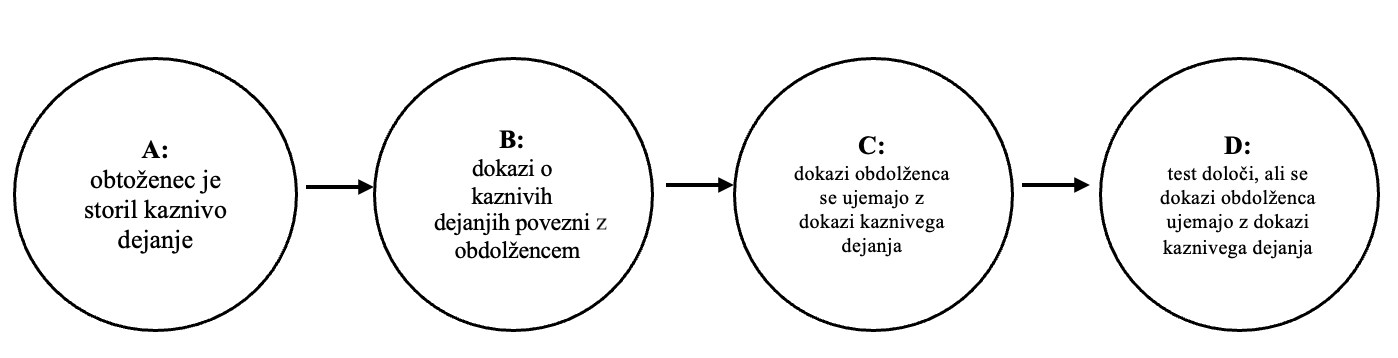
\includegraphics[scale=0.60]{slika_3.png}
   \caption{Vzorčna veriga dokazov}
\end{figure}
\\
Ta analiza je močno odvisna od pojma »pogostost ujemajočih se lastnosti«, označenega kot $F$(lastnosti). Ta se včasih imenuje
tudi »verjetnost naključnega ujemanja«. V našem vzročno-posledičnem okviru je $F$(lastnosti) enakovreden bolj formalno opredeljeni verjetnosti
$P(C \lvert \neg B)$, t.j. verjetnost, da oseba, ki ni vpletena v kaznivo dejanje, po naključju zagotovi dokaze, ki se ujemajo.\\\\
S tem vzročno-posledičnim okvirom lahko opišemo vrsto različnih pogostih zmot, ki so posledica napačnega razumevanja pogojne verjetnosti:\\
\textit{Tožilčeva zmota}: pri tem enačimo $P(C \lvert \neg B)$ s $P(\neg A \lvert C)$. Presega napako predhodne verjetnosti, saj si jo lahko 
predstavljamo kot dopolnitev te napake z dodatno napačno predpostavko $P(A) = P(B)$.\\\\
\textit{Napaka verjetnosti $P(\text{drugo ujemanje})$}: gre za zmoto, ko verjetnost $P(C \lvert \neg B)$ enačimo z verjetnostjo
(imenujmo jo $q$), da ima vsaj en nedolžen član populacije ustreza dokazom. Posledica te napake je običajno močno pretiravanje z vrednostjo
dokaza $C$.\\\\
\textit{Zanemarjanje predhodnih verjetnosti}: to pomeni preprosto neupoštevanje predhodnih vrednosti, kot sta $P(A)$ in $P(B)$. Na splošno
se za zmoto zanemarjanja osnovne stopnje šteje, kadar je verjetnost dogodka podcenjena, ker dogodek ni tako nenavaden, kot se zdi,
ali precenjena, ker je dogodek bolj nenavaden, kot se zdi.\\\\
\textit{Napaka pri številčnem preračunavanju}: pri tem gre za zamenjavo vrednosti $P(C \lvert \neg B)$ s pričakovanim številom drugih oseb,
ki bi jih bilo treba testirati, preden bi našli ujemanje. Ta zmota prav tako pretirava z vrednostjo dokaza $C$.\\\\
\textit{Pričakovane vrednosti, ki pomenijo edinstvenost}: če je velikost populacije približno enaka $1/P(\neg B \lvert C)$, potem mora biti
obdolženec edini primerek. Binomski izrek pokaže, da obstaja več kot 25\% verjetnost, da bosta v populaciji, katere velikost je $1/P(\neg B \lvert C)$,
vsaj dva ujemanja.\\\\
\textit{Zmota obrambnega odvetnika}: to se zgodi, ko se dokaz $C$ šteje za nepomembnega, ker visoka predhodna verjetnost $P(\neg A)$ (kar
se zgodi, če je na primer potencialno število osumljencev zelo veliko) še vedno povzroči visoko verjetnost $P(\neg B \lvert C)$. \\\\
\textit{Napaka baze podatkov obrambnega odvetnika}: za to napako gre, kadar verjetnost $P(\neg B \lvert C)$ temelji na drugačni populaciji,
kot jo določa $P(B)$ ali $P(A)$.\\\\
\textit{Zasliševalčeva zmota}: v tem primeru je dokaz neposredno priznanje krivde. Če to ni potrjeno, to pomeni, da uporabljamo $P(D \lvert A)$ za
informiranje $P(A \lvert D)$. Napaka je, da ne upoštevamo $P(D \lvert \neg A)$. Če je $P(D \lvert A) \leq P(D \lvert \neg A)$, potem dokaz
nima vrednosti.\\\\
Poleg zmot, ki izhajajo iz osnovnega nerazumevanja pogojne verjetnosti, se druge zmote pojavijo zaradi neustreznega združevanja vpliva več dokazov:\\
\textit{Zmota odvisnih dokazov}: ta zmota, ki se včasih imenuje tudi dvojno štetje, se kaže v tem, da se dva ali več dokazov, ki so odvisni,
obravnava, kot da bi bili neodvisni, zaradi česar je izjava o njihovi skupni verjetnosti manjša, kot bi morala biti. Poseben primer te zmote je
\textit{logično odvisna dokazna zmota}, pri kateri en dokaz ni preprosto odvisen od drugega, ampak dejansko logično izhaja iz njega.\\\\
\textit{Napaka konjunkcije}: ta zmota se pojavi, kadar preiskovalec ne upošteva dejstva, da je dokaz sestavljen iz več kot enega negotovega dogodka,
in mu posledično pripiše večjo verjetnost, kot bi jo moral.

--------------------------------------
%%%%%%%%%%%%%%%%%%%%%%%%%%%%%%%%%%%%%%%%%%%%%%%%%%%%%%%%%%%%%%%%%%%%%%%%%%%%%%%%%%%%%%%%%%%%%%%%%%%%%%%%%%%%%%%%%%%%%%%%%%%%%%%%%%%%%%%%%%%%%%
%%%%%%%%%%%%%%%%%%%%%%%%%%%%%%%%%%%%%%%%%%%%%%%%%%%%%%%%%%%%%%%%%%%%%%%%%%%%%%%%%%%%%%%%%%%%%%%%%%%%%%%%%%%%%%%%%%%%%%%%%%%%%%%%%%%%%%%%%%%%%%
\section{Načini za izogib zmotam}
V zadnjih letih je statistika in verjetnost v kazenskem pravu napredovala. Sodniki, tožilstvo in porota se zavedajo nerazumevanja te znanosti, zato 
je statistika čedalje bolj vpletena že v učne programe pravnih fakultet, kar pripomore k boljšemu razumevanju statističnih analiz. Kljub temu so seveda 
zmote še vedno prisotne. V začetku dela sem omenila, da je razlaga statistične analize odvisna od vprašanj odvetnika, pri čemer veliko za izboljšanje 
ne moremo storiti. Poleg tega morajo biti statistični oziroma forenzični znanstveniki previdni z razlago, kajti ne smejo poseči v poroto. Torej kako 
se dejansko izognimo zmotam in s tem ne posežemo v pravna pravila na sodiščih. 

%%%%%%%%%%%%%%%%%%%%%%%%%%%%%%%%%%%%%%%%%%%%%%%%%%%%%%%%%%%%%%%%%%%%%%%%%%%%%%%%%%%%%%%%%%%%%%%%%%%%%%%%%%%%%%%%%%%%%%%%%%%%%%%%%%%%%%%%%%%%%%
\subsection{Izogib zmotam z uporabo razmerja verjetnosti}
Vsem zgoraj opisanim zmotam je skupno to, da je resnična koristnost dokaza predstavljena na zavajajoč način - bodisi je pretirana bodisi podcenjena.
Prednost uporabe razmerja verjetnosti je, da odpravlja ugovor Bayesovemu izreku, in sicer upoštevanje predhodne verjetnosti za hipotezo,
kot je »kriv«. V veliki meri pomiri pomisleke pravnikov, ki bi sicer zavrnili Bayesov argument z utemeljitvijo, da je nedopustno predpostavljati 
predhodne verjetnosti o krivdi ali nedolžnosti.\\\\
Čeprav je uporaba razmerja verjetnosti kot sredstva za izogibanje zmotam in merjenje uporabnosti dokazov močno podprta, sem vseeno mnenja, da
imajo, po prebiranju različnih sodb, pravniki in laiki pogosto podobne težave pri razumevanju razmerja verjetnosti kot pri razumevanju
Bayesove teorije. 

%%%%%%%%%%%%%%%%%%%%%%%%%%%%%%%%%%%%%%%%%%%%%%%%%%%%%%%%%%%%%%%%%%%%%%%%%%%%%%%%%%%%%%%%%%%%%%%%%%%%%%%%%%%%%%%%%%%%%%%%%%%%%%%%%%%%%%%%%%%%%%
\subsection{Izogibanje zmotam z uporabo Bayesovih omrežij}
Ker je največkrat težava v tem, da se večina odvetnikov in sodnikov ob pogledu na verjetnostne izračune in statistično analizo dokazov, ustraši, se mi 
zdijo Bayeosova omrežja dober predlog za predstavitev verjetnostnih izračunov. \\\\
Bayesova omrežja pomagajo določiti ustrezne verjetnostne formule, ne da bi prikazali njihovo polno algebrsko obliko, in omogočajo
skoraj popolno avtomatizacijo potrebnih verjetnostnih izračunov.\\\\
Bayesova omrežja, ki temeljijo na Bayesovi teoriji in teoriji grafov, ponujajo forenzičnim znanstvenikom več prefinjenih možnosti. Tem metodam
se daje poseben poudarek, kadar je treba med konkurenčnimi hipotezami izbrati najverjetnejšo, izbira pa mora biti podprta z znanstveno utemeljeno
argumentacijo. Primerna so za analizo dogodka, ki se je zgodil, in napovedovanje verjetnosti, da je k temu prispeval katerikoli od več možnih
znanih vzrokov. Prednosti Bayesovih mrež se najbolj izrazito pokažejo na zapletenih področjih z več spremenljivkami. Kriminalistične aplikacije
Bayesovih omrežij segajo od prepoznavanja storilcev, posameznih in kompleksnih konfiguracij različnih vrst sledi ter problemov sklepanja, ki
vključujejo rezultate analiz DNK.\\
Ti grafični modeli verjetnosti bistveno izboljšajo vrednotenje verjetnostnih razmerij, ki se uporabljajo za ocenjevanje znanstvenih dokazov.
Omogočajo, da se lotimo kompleksnejših verjetnostnih analiz, kot bi bilo to mogoče s tradicionalnimi pristopi, kar še posebaj pride prav pri primerih z ogromno doazi. \\\\
Struktura Bayesovega omrežja v pravnem kontekstu je dovzetna za napačne predpostavke in napake v procesu ustvarjanja. Izbira vozlišč za dokaze je lahko
pristranska glede na to, kakšna vrsta argumenta je predstavljena. Argumenti obrambe ali tožilstva lahko na primer poudarjajo nasprotne sklepe
in zato vključujejo le podskupino dokazov. Če se za izdelavo ne uporablja dosleden okvir, lahko Bayesovo omrežje, ki jih oblikujejo različne stranke za en
primer, kažejo različne rezultate. Pri oblikovanju Bayesovega omrežja za pravno sklepanje ključnega pomena, da se oblikuje omrežje, ki je razumljivo poroti
in sodniku.\\\\
Prikaz Bayesovega omrežja se mora ujemati z intuitivnim pripisovanjem vzročno-posledičnih povezav med končno hipotezo, kot je »Obtoženec je kriv.«, podhipotezo
»Obtoženec je bil na kraju zločina.« in dokazi primera. Poleg težav, ki se pojavijo med postopkom strukturiranja, je problematično tudi sklepanje
iz omrežja, če se izvaja ob napačnih predpostavkah. Verjetnosti, tudi če temeljijo na strokovni presoji, so lahko pristranske zaradi dejavnikov
motenj v postopku pridobivanja podatkov. Metode za sklepanje morajo zato zagotoviti, da se verjetnosti omrežij ne razlagajo napačno kot dejstva in
da se izpostavi dejavnik negotovosti. Primerjati morajo verjetnosti za nasprotujoče si hipoteze in morajo zagotoviti okvir za pravnike, da iz
mreže sklepajo na argumente.

%%%%%%%%%%%%%%%%%%%%%%%%%%%%%%%%%%%%%%%%%%%%%%%%%%%%%%%%%%%%%%%%%%%%%%%%%%%%%%%%%%%%%%%%%%%%%%%%%%%%%%%%%%%%%%%%%%%%%%%%%%%%%%%%%%%%%%%%%%%%%%
%%%%%%%%%%%%%%%%%%%%%%%%%%%%%%%%%%%%%%%%%%%%%%%%%%%%%%%%%%%%%%%%%%%%%%%%%%%%%%%%%%%%%%%%%%%%%%%%%%%%%%%%%%%%%%%%%%%%%%%%%%%%%%%%%%%%%%%%%%%%%%
\section{Zaključek}

\end{document}